%%%%%%%%%%%%%%%%%%%%%%%%%%%%%%%%%%%%%%%%%%%%%%%%%%%%%%%%%%%%%%%%%%%%%%
% How to use writeLaTeX: 
%
% You edit the source code here on the left, and the preview on the
% right shows you the result within a few seconds.
%
% Bookmark this page and share the URL with your co-authors. They can
% edit at the same time!
%
% You can upload figures, bibliographies, custom classes and
% styles using the files menu.
%
%%%%%%%%%%%%%%%%%%%%%%%%%%%%%%%%%%%%%%%%%%%%%%%%%%%%%%%%%%%%%%%%%%%%%%

\documentclass[12pt]{article}
\usepackage{subcaption}
\usepackage{sbc-template}
\usepackage{float}

\usepackage{graphicx,url}

\usepackage{graphicx}

\usepackage[brazil]{babel}   
\usepackage[utf8]{inputenc}  
\usepackage{geometry}
\usepackage{float}
\usepackage{sbc-template}
\usepackage{bera}% optional: just to have a nice mono-spaced font
\usepackage{listings}
\usepackage{xcolor}
\usepackage{booktabs}
\usepackage{verbatim}
\usepackage{amsmath}
     
\sloppy

\title{Implementação e avaliação do algoritmo Merge Sort e de suas variações}

\author{Luís Gustavo Werle Tozevich\inst{1}, Jaime Antonio Daniel Filho\inst{1}, Guilherme M. Einloft\inst{1}}
\address{Curso de Ciência da Computação, Universidade Federal de Santa Maria
  (UFSM)\\
  \email{lgtozevich@inf.ufsm.br, jafilho@inf.ufsm.br, guieinloft@proton.me}
}
\begin{document} 

\maketitle

\section{Introdução}

% A ordenação de dados é uma operação fundamental na área da computação, influenciando significativamente a eficiência de sistemas que gerenciam grandes volumes de informações. 

Em um mundo cada vez mais orientado por dados, a capacidade de ordenar informações de maneira rápida e eficaz é crucial para o desempenho de diversas aplicações, desde bancos de dados que precisam acessar registros rapidamente até algoritmos de busca que dependem de conjuntos ordenados para encontrar resultados relevantes. Desse modo, a escolha do algoritmo de ordenação adequado pode resultar em economias substanciais de tempo e de recursos, impactando diretamente a experiência do usuário e a escalabilidade dos sistemas.

Este trabalho tem como objetivo implementar e comparar diferentes algoritmos de ordenação utilizando a linguagem C, com o intuito de investigar os atributos exclusivos inerentes a cada método. Os algoritmos designados para análise incluem \textit{Merge Sort} (em suas formas iterativa, recursiva e paralela), \textit{Quicksort}, \textit{Insertion Sort} e o híbrido \textit{Quicksert}, cada um apresentando características distintas relacionadas à complexidade computacional, utilização de memória e eficiência em diferentes contextos de distribuição de dados. A implementação desses algoritmos será realizada de forma a permitir a avaliação da eficiência em variados conjuntos de dados e, consequentemente, a comparação do desempenho prático em relação ao teórico.

Por meio dos experimentos realizados, será possível observar não apenas o tempo de execução de cada algoritmo, mas também o impacto de diferentes organizações de dados em implementações específicas. Isso permitirá identificar qual algoritmo se adapta melhor a diferentes situações, contribuindo para o entendimento das suas características e suas aplicações em contextos práticos.

\section{\textit{Merge Sort}}

O algoritmo \textit{Merge Sort}, proposto por John von Neumann em 1945, é uma implementação paradigmática da estratégia de divisão e conquista (\textit{divide-and-conquer})\footnote{Consiste em dividir um problema complexo em subproblemas menores e independentes, resolve-los recursivamente e combinar as soluções para obter a resposta final}, amplamente adotado para a ordenação de dados em diversas áreas da ciência da computação. A operação central do algoritmo consiste em dividir recursivamente um vetor em subvetores até que cada subvetor contenha um único elemento. Em seguida, realiza-se a fusão (\textit{merge}) dos subvetores, ordenando-os de maneira crescente ou decrescente, conforme o critério especificado, até que todos os elementos estejam organizados em um único vetor ordenado, como ilustrado na Figura \ref{fig:arvore}. Esse processo permite que o algoritmo atinja uma complexidade temporal de $O(n\log{n})$, sendo uma escolha eficiente para cenários que envolvem grandes volumes de dados e, consequentemente, justificando sua implementação em bibliotecas de linguagens de programação e sistemas operacionais [SARA et al., 2019; SINGH \& SINGH, 2014].


\begin{figure}[H] \caption{Ilustração do processo de divisão e de conquista do algoritmo \textit{Merge Sort}} \centering 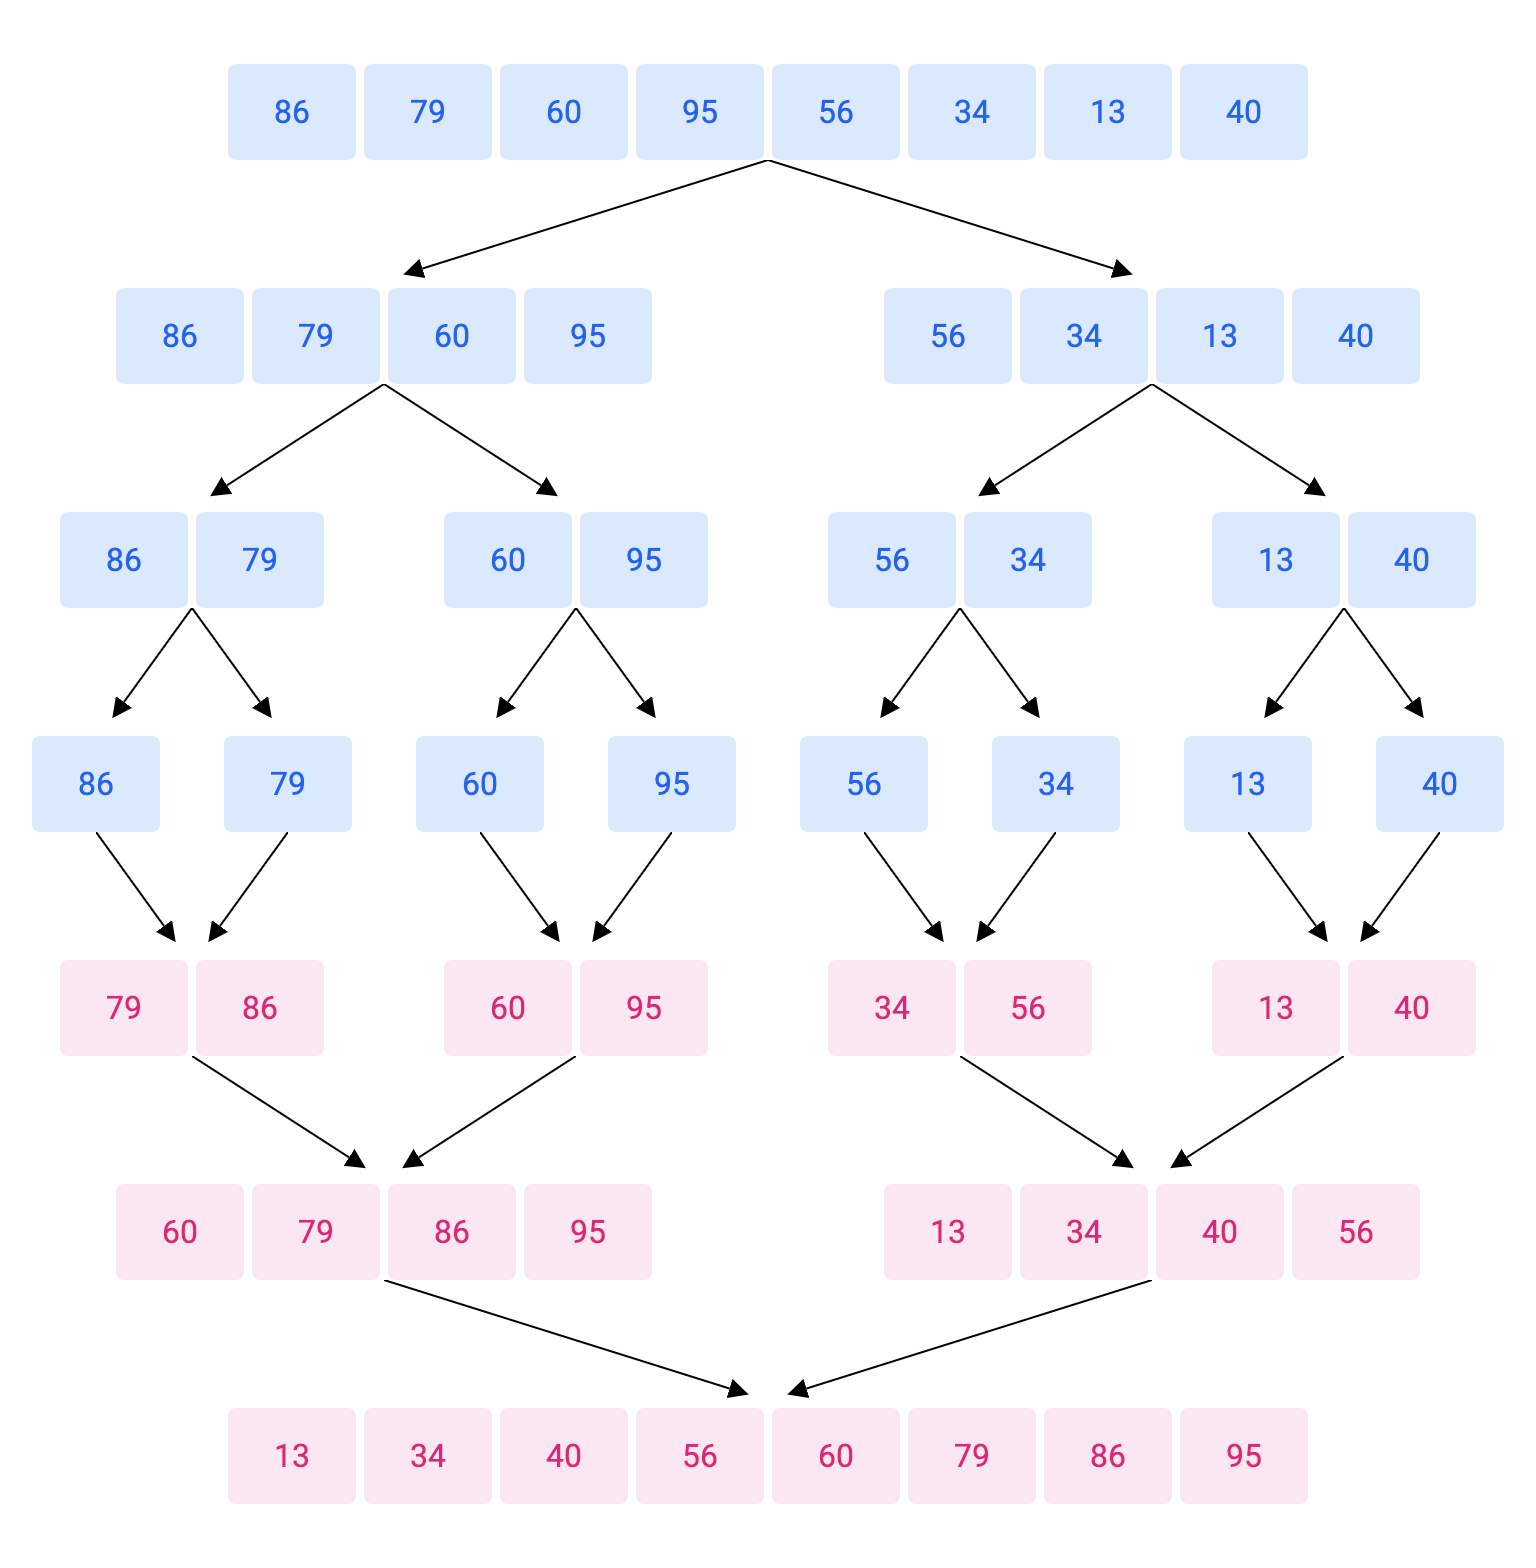
\includegraphics[width=0.7\textwidth]{visualization.png}  \label{fig:arvore} \end{figure}

Uma característica do Merge Sort é a estabilidade, ou seja, ele preserva a ordem relativa dos elementos com chaves iguais, o que é uma propriedade essencial em diversas aplicações, especialmente em ordenações secundárias. Outra vantagem é sua capacidade de ser paralelizado com eficiência, permitindo sua adaptação para processamento em múltiplos núcleos e otimizando o desempenho em sistemas que demandam alta performance [SARA et al., 2019].

O algoritmo também encontra aplicação em contextos que envolvem grandes volumes de dados, como em instituições financeiras que precisam processar extensos fluxos de informações em tempo real [\textit{"A New Optimized Version of Merge Sort"}, 2023]. Além disso, sua versatilidade permite que seja implementado de diferentes formas, como a versão recursiva clássica, uma variante iterativa e uma versão paralelizada para sistemas \textit{multicore}, que serão discutidas nas subseções \ref{recursiva}, \ref{iterativa} e \ref{paralelizada}, respectivamente.

\subsection{Implementação recursiva}\label{recursiva}

A implementação recursiva do \textit{Merge Sort} é a forma canônica do algoritmo e exemplifica de maneira clara o paradigma de divisão e conquista. Nessa abordagem, o vetor de entrada é dividido recursivamente ao meio até que seja obtido um conjunto de subvetores de tamanho unitário. A fase de fusão (\textit{merge}) combina esses subvetores ordenados, retornando um vetor completamente ordenado. A recursão é finalizada quando os subvetores atingem tamanho 1, o que corresponde ao caso base.

Uma das principais vantagens da implementação recursiva é sua simplicidade conceitual e a facilidade com que pode ser descrita e implementada. Entretanto, essa implementação pode resultar em um consumo adicional de memória na pilha de execução proporcional ao logaritmo do número de elementos, ou seja, $\log{n}$, o que pode restringir o tamanho da entrada em sistemas que possuem limitações nesse aspecto. Ainda assim, a complexidade temporal permanece $O(n\log{n})$ em todos os casos.

\subsection{Implementação iterativa}\label{iterativa}

 A implementação iterativa do \textit{Merge Sort} elimina o uso de recursão, substituindo-a por laços iterativos que controlam as divisões e as fusões do vetor. Nessa abordagem, o vetor é subdividido em blocos de tamanho crescente, começando de pares de elementos adjacentes, que são posteriormente fundidos em blocos maiores, até que o vetor inteiro esteja ordenado.

Uma vantagem dessa implementação é o controle explícito sobre o uso de memória, uma vez que elimina a necessidade de uma pilha recursiva. No entanto, a versão iterativa tende a ser um pouco mais complexa em termos de implementação do que a versão recursiva, dado que o controle das divisões e das fusões deve ser manualmente gerido por meio de estruturas de laço. Apesar disso, em termos de complexidade temporal, a versão iterativa do \textit{Merge Sort} também apresenta desempenho de $O(n\log{n})$.


\subsection{Implementação paralelizada}\label{paralelizada}

A implementação paralelizada do \textit{Merge Sort} aproveita as características do algoritmo para ser executado de maneira eficiente em sistemas \textit{multicore} ou multiprocessadores. A fase de divisão pode ser realizada de forma independente em diferentes núcleos, uma vez que essa operação não depende de nenhuma etapa anterior, tornando o algoritmo altamente paralelizável. Da mesma forma, a fusão dos subvetores pode ser distribuída entre diferentes núcleos, desde que o acesso à memória seja adequadamente sincronizado. Dessa forma, embora a complexidade temporal permaneça $O(n\log{n})$, o tempo total de execução pode ser significativamente reduzido, a depender do grau de paralelismo explorado e do tamanho dos dados.

Em nossa implementação, a criação de \textit{threads} ocorre somente quando o vetor ultrapassa 100 mil elementos. Esse valor foi escolhido após uma suíte de testes com diferentes tamanhos de conjuntos de dados, visando equilibrar a sobrecarga da criação de \textit{threads} com o ganho de desempenho proporcionado pelo paralelismo. Isso porque, para conjuntos menores que o limiar, a sobrecarga adicional de criar e gerenciar \textit{threads} não compensava os ganhos de desempenho, tornando a execução sequencial mais eficiente. 

% No entanto, para conjuntos de dados maiores, o limiar escolhido se demonstrou ideal, oferecendo uma melhoria significativa na redução do tempo de execução.

% Em termos de desempenho, a versão paralelizada do Merge Sort pode alcançar uma redução substancial no tempo de execução em sistemas com múltiplos núcleos, especialmente em grandes conjuntos de dados. Dessa forma, embora a complexidade temporal permaneça $O(n\log{n})$, o tempo total de execução pode ser significativamente reduzido, a depender do grau de paralelismo explorado e do tamanho dos dados.

% O ganho de desempenho depende diretamente da eficiência do controle de paralelismo e da infraestrutura subjacente, como o uso de bibliotecas de paralelização, por exemplo, pthreads, OpenMP ou MPI.
   
\section{Outros algoritmos para comparação}

Neste capítulo, descreveremos os algoritmos implementados e utilizados para comparação entre as diferentes versões do \textit{Merge Sort}. A tabela \ref{table:alg_comp} apresenta os algoritmos implementados e suas respectivas complexidades em cada caso de uso.

\begin{table}[htpb]
\centering

\caption{Complexidade dos algoritmos analisados}
\begin{tabular}{c c c c c c}
\toprule
Algoritmo & Melhor caso & Caso Médio & Pior Caso\\
\midrule
Merge Sort & $O(n \log n)$ & $O(n \log n)$ & $O(n \log n)$ \\
Insertion Sort &$O(n)$ & $O(n^2)$  & $O(n^2)$\\
Quicksort & $O(n \log n)$ & $O(n \log n)$ & $O(n^2)$ \\
Quicksert & $O(n \log n)$ & $O(n \log n)$ & $ O(n^2)$ \\
\bottomrule
\end{tabular}
\label{table:alg_comp}
\end{table}

\subsection{\textit{Insertion Sort}}

O \textit{Insertion Sort}  é o método comumemente usado por jogadores para ordenar as suas cartas de baralho [Bentley, 2000]. Eles guardam as cartas que já receberam de maneira ordenada em uma de suas mãos e inserem cada nova carta recebida na posição apropriada. Computacionalmente, a ordenação ocorre de forma iterativa, iniciando o vetor ordenado com o primeiro elemento do vetor de partida. Em seguida, retira-se o próximo elemento do vetor de partida, encontra-se a sua posição no vetor ordenado e o insere na posição encontrada. Isso é realizado até não haja mais elementos restantes no vetor de partida. Dessa forma, o \textit{Insertion Sort} atinge a complexidade de tempo de $O(n^2)$ no pior caso e no caso médio e de $O(n)$ no melhor caso. No entanto, apesar dessa elevada complexidade de tempo em comparação com outros algoritmos, a sua execução costuma ser substancialmente mais rápida para conjuntos com uma baixa quantidade de elementos [Cormen et al., 2022].

\subsection{\textit{Quicksort}}

O \textit{Quicksort} alcança a complexidade de tempo de $O(n^2)$ no pior caso e $O(n\log{n})$ tanto no caso médio quanto no melhor caso, por meio do método da divisão e conquista [Cormen et al., 2022]. Nesse algoritmo, o vetor inicial é particionado em dois subvetores com base na escolha de um elemento pivô, de modo que um subvetor contenha os elementos menores que o pivô e o outro subvetor contenha os elementos maiores que o pivô. Isso é repetido até que todos os subvetores sejam de tamanho 1, estando, desse modo, ordenados trivialmente. Após essa etapa, basta juntar os subvetores para obter o vetor final ordenado.

\subsection{\textit{Quicksert}}  \label{sec:firstpage}

O \textit{Quicksert} combina o \textit{Quicksort} e o \textit{Insertion Sort} em um algoritmo de ordenação híbrida, visando mitigar as desvantagens individuais de cada algoritmo e obter um melhor desempenho em conjuntos de dados variados. Nesse sentido, é importante considerar que, embora o \textit{Quicksort} tenha uma complexidade temporal média menor que o \textit{Insertion Sort}, ele apresenta uma sobrecarga significativamente maior, devido à sua natureza recursiva, a qual o torna menos eficiente para vetores pequenos. Ademais, ambos algoritmos podem se degenerar para um tempo de execução quadrático, sob certas condições dos dados de entrada.

O algoritmo híbrido \textit{Quicksert} tem como objetivo sanar as observações supracitadas. Sua execução inicia-se com o particionamento do \textit{Quicksort}, porém, ao invés de continuar até alcançar subvetores de tamanho 1, a operação é interrompida quando os subvetores atingem um tamanho menor ou igual a um determinado limiar. O vetor resultante será constituído de subvetores de tamanho menor ou igual ao limiar, os quais, apesar de não estarem ordenados internamente, estão na ordem correta em relação uns aos outros. Para concluir a ordenação, o \textit{Insertion Sort} é aplicado sobre o vetor parcialmente ordenado, produzindo o vetor totalmente ordenado. Com essa implementação, o algoritmo híbrido atinge a complexidade temporal de $O(n^2)$ no pior caso e de $O(n\log{n})$ no caso médio e no melhor caso.

Por fim, em virtude da efetividade do \textit{Quicksert} depender majoritariamente do limiar escolhido, isto é, do tamanho superior dos vetores nos quais serão aplicados o \textit{Insertion Sort}, realizou-se uma grande quantidade de testes para encontrar o limiar ideal. Com base nos resultados, concluiu-se que o valor 23 é a melhor escolha para o limiar, pois obteve o menor tempo médio de execução em comparação com o restante dos limiares.

\section{Análise e comparação de algoritmos}

Os algoritmos foram avaliados em três cenários: dados em ordem crescente, dados aleatórios e dados em ordem decrescente. Os testes foram realizados utilizando um programa para o medir o tempo de execução para a ordenação dos dados. Cada algoritmo foi submetido a diferentes tamanhos de conjunto, variando de 0 até 10 milhões de elementos com incrementos de 100 mil. O \textit{Insertion Sort}, devido ao seu desempenho no caso médio e no pior caso, foi testado apenas até 100 mil elementos para o conjunto de dados aleatório e para o conjunto de dados em ordem decrescente. Cada ordenação foi executada 100 vezes para cada algoritmo e cada cenário, e os valores apresentados nos gráficos representam a média dos resultados obtidos.

A Figura \ref{fig:asc} ilustra o melhor caso, isto é, quando o conjunto de dados está previamente ordenado. Nesse cenário, como mostrado na figura, o algoritmo \textit{Insertion Sort} apresentou o menor tempo médio de ordenação, seguido pelo \textit{Merge Sort} paralelo. O \textit{Quicksort}, por sua vez, obteve o pior tempo médio. Isso ocorre porque, ao lidar com dados previamente ordenados, o algoritmo \textit{Quicksort} pode se degenerar para seu pior caso de complexidade, $O(n^2)$, dependendo da escolha do elemento pivô. Nessa situação, a partição dos elementos não é equilibrada, e o algoritmo acaba gerando divisões extremamente desbalanceadas, em que uma das partições contém quase todos os elementos e a outra, quase nenhum. Assim, em vez de dividir o problema de forma eficiente, o \textit{Quicksort} realiza muitas comparações desnecessárias, aumentando o tempo de execução.

\begin{figure}[ht]
\centering
\caption{Tempo de execução com dados crescentes}
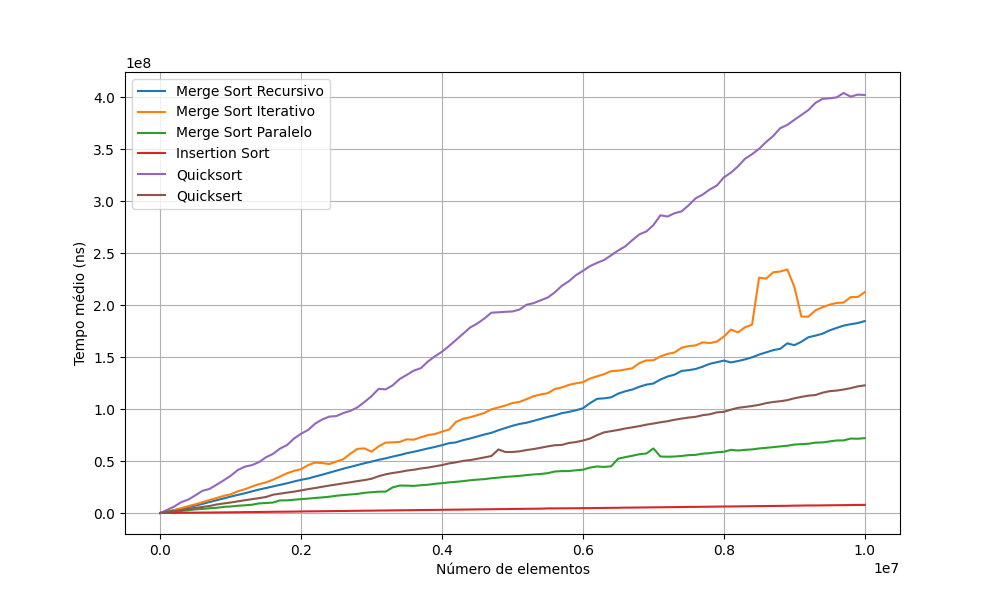
\includegraphics[width=0.85\textwidth]{time_ascending.png}
\label{fig:asc}
\end{figure}

Em contrapartida, a Figura \ref{fig:desc} evidencia o pior caso para um conjunto de dados, onde os dados estão dispostos em ordem inversa. Nesse cenário, ao contrário do primeiro caso, o algoritmo \textit{Insertion Sort} apresentou o pior resultado, não conseguindo ordenar mais de 100 mil elementos no tempo estipulado devido a sua complexidade quadrática. Além disso, o \textit{Quicksort} também teve seu desempenho prejudicado pela natureza dos dados.

Ademais, ao analisarmos a Figuras \ref{fig:asc} e a Figura \ref{fig:desc}, percebe-se que o algoritmo híbrido \textit{Quicksert} apresentou uma vantagem em relação aos métodos convencionais de ordenação. Ele obteve bons resultados devido à sua integração com o \textit{Insertion Sort}, sendo mais eficiente que seus algoritmos individuais.

\begin{figure}[ht]
\centering
\caption{Tempo de execução com dados decrescentes}
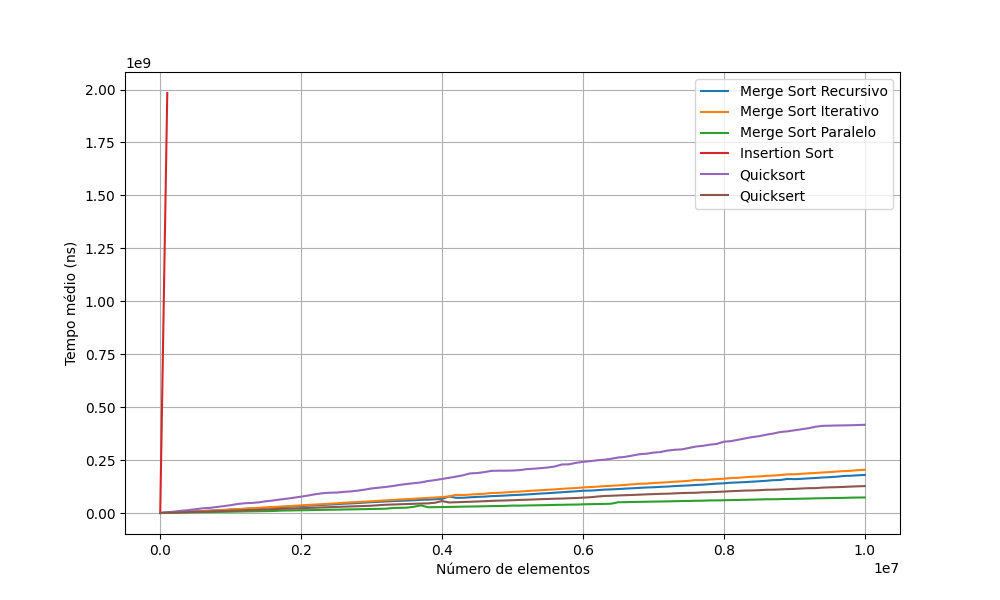
\includegraphics[width=0.85\textwidth]{time_descending.png}
\label{fig:desc}
\end{figure}


Outrossim, a Figura \ref{fig:rand} ilustra um dos cenários mais comuns de ordenação de dados, em que os elementos não apresentam qualquer ordenação prévia, caracterizando o caso médio dos algoritmos implementados. Da mesma forma que observado na Figura \ref{fig:desc}, o \textit{Insertion Sort} revela-se uma escolha inadequada para conjuntos de dados grandes, exigindo mais tempo para ordenar 100 mil elementos do que os demais algoritmos para ordenar 10 milhões de elementos. Nesse contexto, o \textit{Quicksert} destaca-se novamente como a alternativa mais eficiente na ausência de paralelização. No entanto, ao considerarmos a paralelização, o \textit{Merge Sort} demonstrou ser capaz de lidar com grandes volumes de dados de forma eficaz em todos os cenários analisados.

\begin{figure}[ht]
\centering
\caption{Tempo de execução com dados aleatórios}
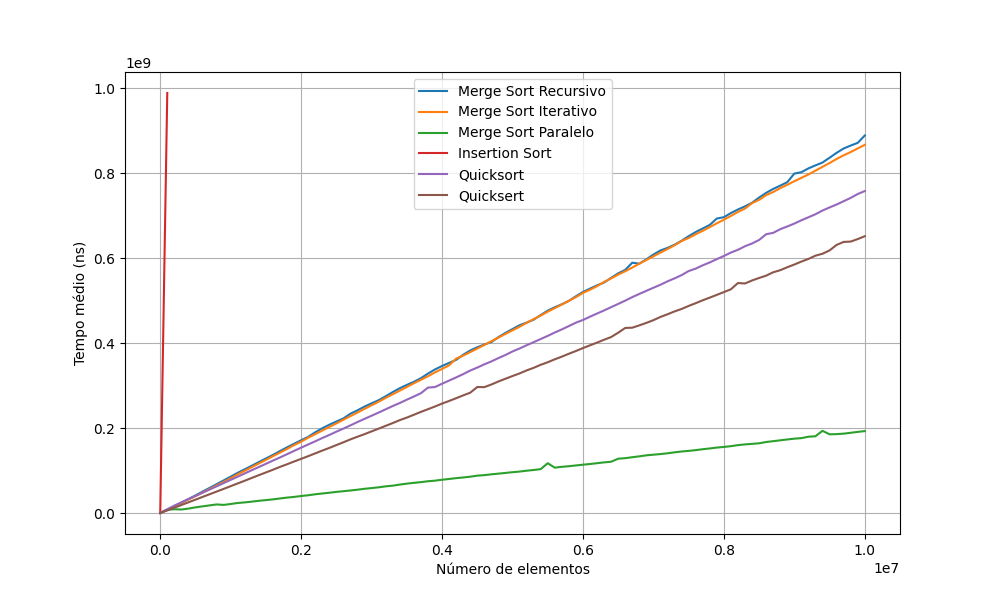
\includegraphics[width=0.85\textwidth]{time_random.png}
\label{fig:rand}
\end{figure}

Em suma, com base nas figuras analisadas, podemos concluir que o \textit{Merge Sort} apresenta resultados consistentes independentemente da ordem inicial dos dados, devido à sua complexidade de tempo invariável em todos os casos, o que torna seu desempenho previsível. Nesse sentido, tanto as implementações recursivas quanto as iterativas mantêm a mesma eficiência, sendo a escolha entre elas mais uma questão de estilo de codificação ou restrições da plataforma, como a profundidade da pilha, sem impactar a complexidade final. A adição de paralelização ao \textit{Merge Sort} proporciona uma melhora drástica no tempo de execução ao aproveitar múltiplos núcleos de processamento, em contraste com algoritmos sequenciais, sem aumentar significativamente a complexidade de implementação.

Em comparação, os demais algoritmos, embora não sejam tão previsíveis quanto o \textit{Merge Sort}, destacam-se em cenários específicos. O \textit{Insertion Sort}, por exemplo, é eficiente em dados quase ordenados, devido à sua simplicidade e baixa sobrecarga, mas sua complexidade quadrática prejudica o desempenho em conjuntos grandes ou inversamente ordenados. Já o \textit{Quicksort}, com sua abordagem de divisão e conquista, oferece excelente desempenho no caso médio, especialmente com dados aleatórios, mas pode se degenerar para uma complexidade quadrática, como em dados ordenados de forma crescente ou decrescente, dependendo do pivô escolhido. Por fim, o algoritmo híbrido \textit{Quicksert}, que combina a rapidez do \textit{Quicksort} com a simplicidade do \textit{Insertion Sort} para subproblemas menores, demonstrou ser uma solução eficiente em diversos cenários, maximizando o desempenho com diferentes tipos de dados e evitando as desvantagens críticas dos outros dois algoritmos individuais.

% Portanto, com base nas Figuras analisadas, podemos concluir que o Merge Sort apresenta resultados consistentes, independentemente da ordem inicial dos dados, devido à sua complexidade de tempo invariável em todos os casos, o que torna seu desempenho previsível. Tanto as implementações recursivas quanto iterativas do Merge Sort mantêm a mesma eficiência, sendo a escolha entre elas mais uma questão de estilo de codificação ou restrições da plataforma, como a profundidade da pilha, sem impactar o a complexidade final. A adição de paralelização ao Merge Sort, por sua vez, propicia uma melhora drástica no tempo de execução, aproveitando eficientemente múltiplos núcleos de processamento, em contraste com os algoritmos sequenciais.

% Outrossim, notemos que os demais algoritmos, apesar de não serem previsíveis como o Merge Sort, destacam-se em cenários específicos. O Insertion Sort é eficiente em casos onde os dados já estão quase ordenados, devido à sua simplicidade e baixa sobrecarga. No entanto, sua complexidade quadrática faz com que seu desempenho caia drasticamente em conjuntos grandes ou em ordem inversa. O Quicksort, com sua abordagem de divisão e conquista, oferece excelente desempenho no caso médio, especialmente com dados aleatórios, mas pode ser prejudicado no pior caso, como em dados ordenados de forma crescente ou decrescente, dependendo da escolha do pivô. Por outro lado, o algoritmo híbrido Quicksert, que combina a rapidez do Quicksort com a simplicidade do Insertion Sort para subproblemas menores, demonstrou ser uma solução eficiente em diferentes cenários, maximizando o desempenho em diversos tipos de dados, sem as desvantagens críticas dos outros dois algoritmos.

% Outrossim, o Insertion Sort, o Quicksort e o Quicksert. O Insertion Sort é eficiente em conjuntos pequenos ou parcialmente ordenados, apresentando excelente desempenho no melhor caso, onde sua complexidade é linear ($O(n)$). No entanto, seu desempenho degrada rapidamente com o aumento do número de elementos ou em cenários de dados desordenados, devido à sua complexidade quadrática no caso médio e pior ($O(n^2)$). O Quicksort, por outro lado, brilha em dados aleatórios ou ligeiramente desordenados, oferecendo um desempenho médio de $O(n \log n)$, mas é penalizado severamente em seu pior caso ($O(n^2)$) quando lida com dados já ordenados ou inversamente ordenados, se o pivô não for bem escolhido. O Quicksert, sendo um algoritmo híbrido que combina as características do Insertion Sort e do Quicksort, se sobressai pela capacidade de adaptar-se ao tamanho e ordenação dos dados, mantendo eficiência nos cenários onde seus algoritmos base isoladamente apresentam limitações. Ele proporciona uma solução equilibrada, com um desempenho robusto mesmo em conjuntos grandes, destacando-se como uma alternativa versátil e eficaz para uma variedade de situações.

% Por outro lado, os demais algoritmos se sobressaem em cenários específicos. O Insertion Sort, por exemplo, destaca-se em vetores ordenados, demandando um número mínimo de operações para manter a ordem, ao passo que o Quicksort 

% Além disso, o Insertion Sort, embora ineficiente para dados aleatórios devido ao seu comportamento em conjuntos desordenados, sobressai-se em vetores já ordenados, demandando um número mínimo de operações para manter a ordem. Por outro lado, como supracitado, o Quicksort ainda se destaca como o mlehor algoritmo sem paralelização para cenários que os dados estejam em ordem aleatória. apresenta desempenho inferior quando aplicado a dados inicialmente ordenados, independentemente da direção. No entanto, ele ainda se destaca como o melhor algoritmo convencional sem paralelização para cenários que os dados estejam em ordem aleatória. No entanto, ao combinar o Quicksort com o Insertion Sort em subvetores pequenos, maximiza-se a eficiência deste último, facilitando o tratamento rápido de conjuntos menores, surgindo assim o Quicksert.

\subsection{Análise da relação entre complexidade teórica e prática}

A notação O é uma forma de descrever o comportamento assintótico de uma função.  Dizemos que uma função $f(n)$ é $O(g(n))$ se, para valores suficientemente grandes de $n$, $f(n)$ é limitada superiormente por uma constante vezes $g(n)$. Ou seja, existe uma constante positiva $c$ e um valor $n_0$ tal que:

$$
f(n) \leq c \cdot g(n) \quad \forall \quad n \geq n_0
$$

Isso implica que existe uma constante $c$ tal que $f(n)$ nunca ultrapassa $c \cdot g(n)$ para valores suficientemente grandes de $n$. Essa constante $c$ pode ser estimada para cada amostra específica ao se dividir o tempo medido pelo tempo esperado. No caso do algoritmo \textit{Merge Sort}, cuja complexidade é limitada superiormente por $O(n \log n)$, como ilustrado na Tabela \ref{table:alg_comp}, podemos calcular essa constante por meio da seguinte equação:

\begin{equation}
\label{eq:constant}
    c = \frac{t_{\text{medido}}}{t_{\text{esperado}}} = \frac{t_{\text{medido}}}{n\log{n}}
\end{equation}

A Figura \ref{fig:asc_c}, a Figura \ref{fig:desc_c} e a Figura \ref{fig:random_c} nos mostram o resultado do cálculo da Equação \ref{eq:constant} para cada tamanho do vetor no caso com dados crescentes, decrescentes e aleatórios para a implementação recursiva, iterativa e paralela. Dessa forma, com base na Figura \ref{fig:asc_c}, na Figura \ref{fig:desc_c} e na Figura \ref{fig:random_c} é possível afirmar que em termos práticos (pelo menos até 10 milhões de elementos) o \textit{Merge Sort} (em todas as implementações e casos) é limitado superiormente por uma constante.

\begin{figure}[H]
    \caption{Constante do Merge Sort com dados crescentes}
    \centering
    \begin{subfigure}{0.49\textwidth}
        \centering
        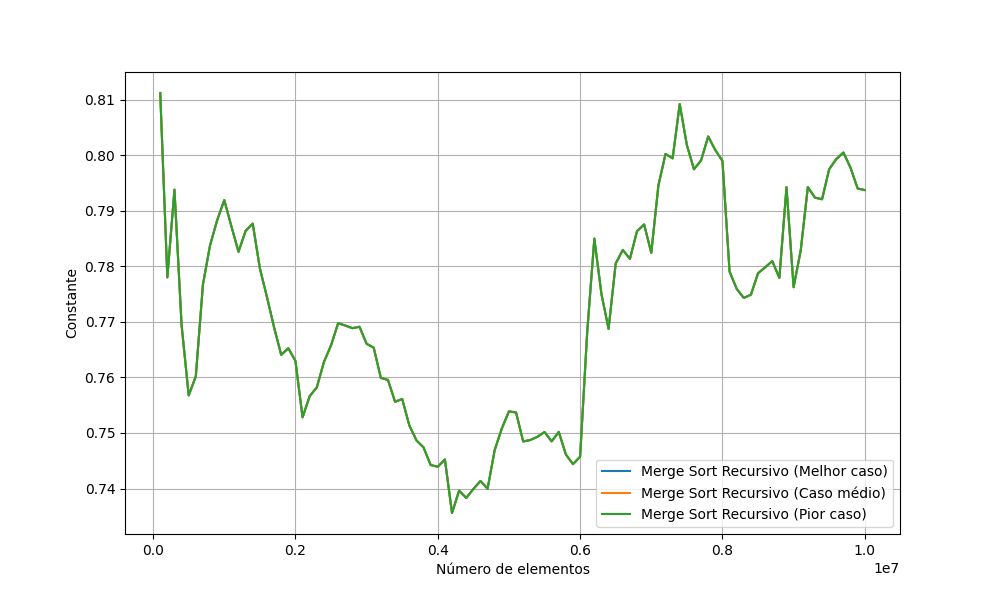
\includegraphics[width=\linewidth]{complexity_ascending_recursive_mergesort.png}
        \label{fig:imagem1}
    \end{subfigure}
    \hfill
    \begin{subfigure}{0.49\textwidth}
        \centering
        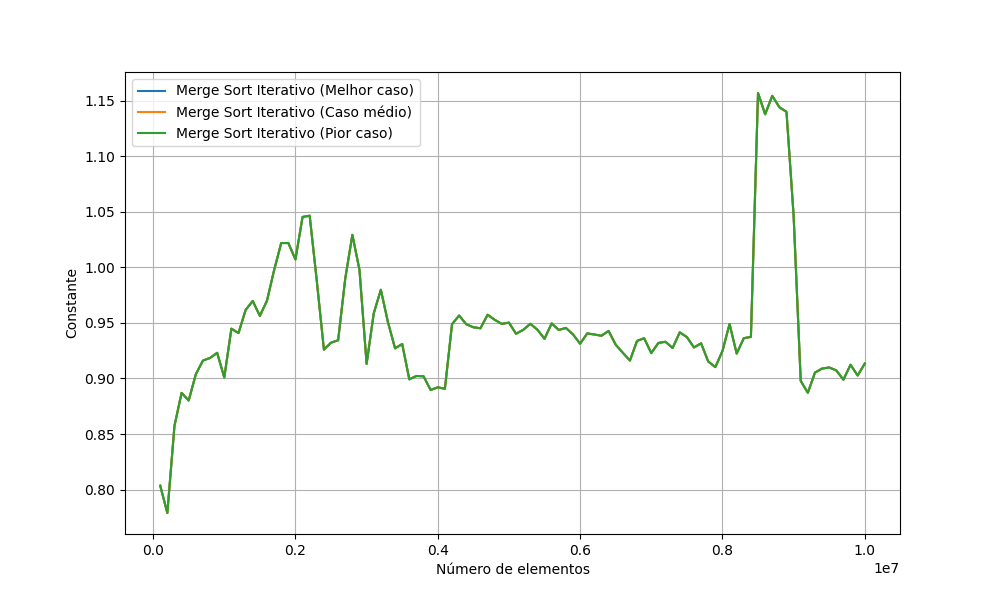
\includegraphics[width=\linewidth]{complexity_ascending_iterative_mergesort.png}
        \label{fig:imagem2}
    \end{subfigure}
    \begin{subfigure}{0.49\textwidth}
        \centering
        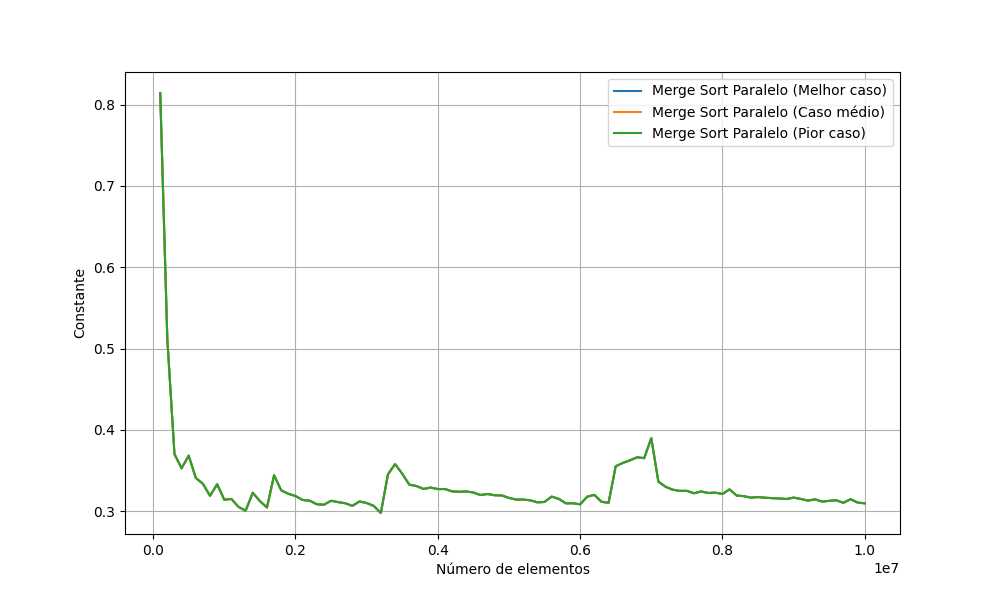
\includegraphics[width=\linewidth]{complexity_ascending_parallel_mergesort.png}
        \label{fig:imagem3}
    \end{subfigure}
    \label{fig:asc_c}
\end{figure}

\begin{figure}[H]
    \caption{Constante do Merge Sort com dados decrescentes}
    \centering
    \begin{subfigure}{0.49\textwidth}
        \centering
        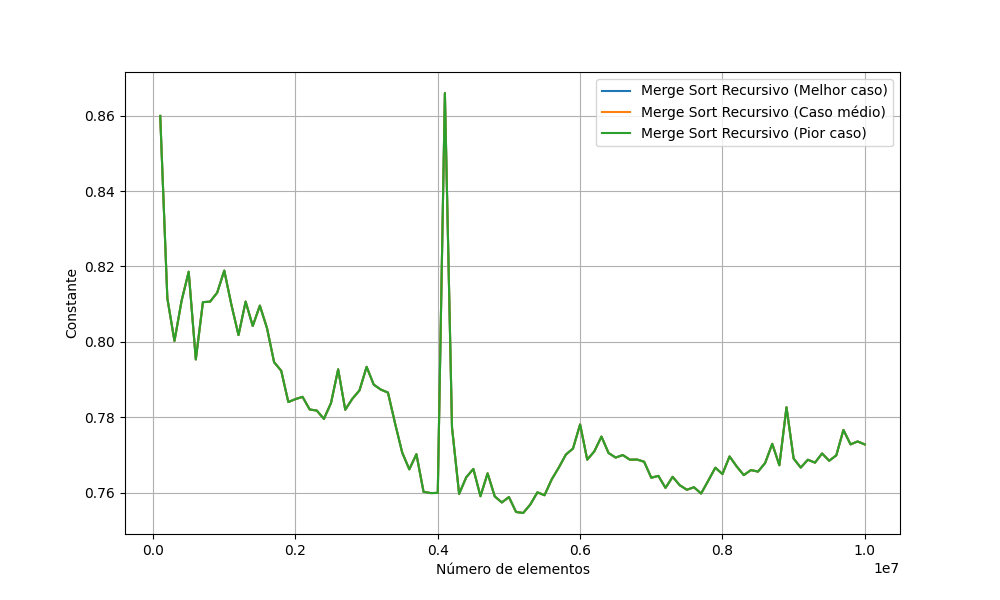
\includegraphics[width=\linewidth]{complexity_descending_recursive_mergesort.png}
        \label{fig:imagem1}
    \end{subfigure}
    \hfill
    \begin{subfigure}{0.49\textwidth}
        \centering
        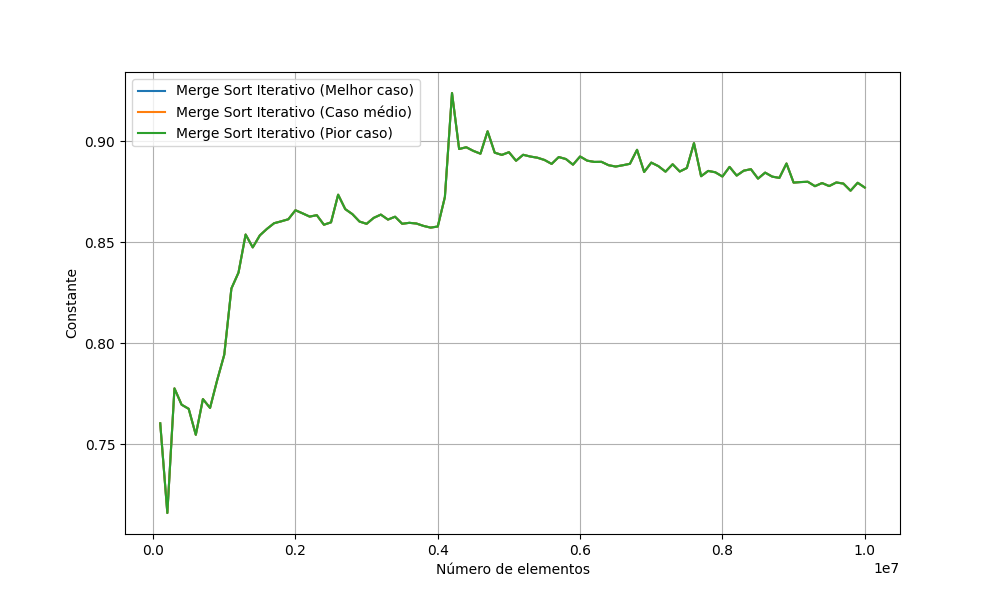
\includegraphics[width=\linewidth]{complexity_descending_iterative_mergesort.png}
        \label{fig:imagem2}
    \end{subfigure}
    \begin{subfigure}{0.49\textwidth}
        \centering
        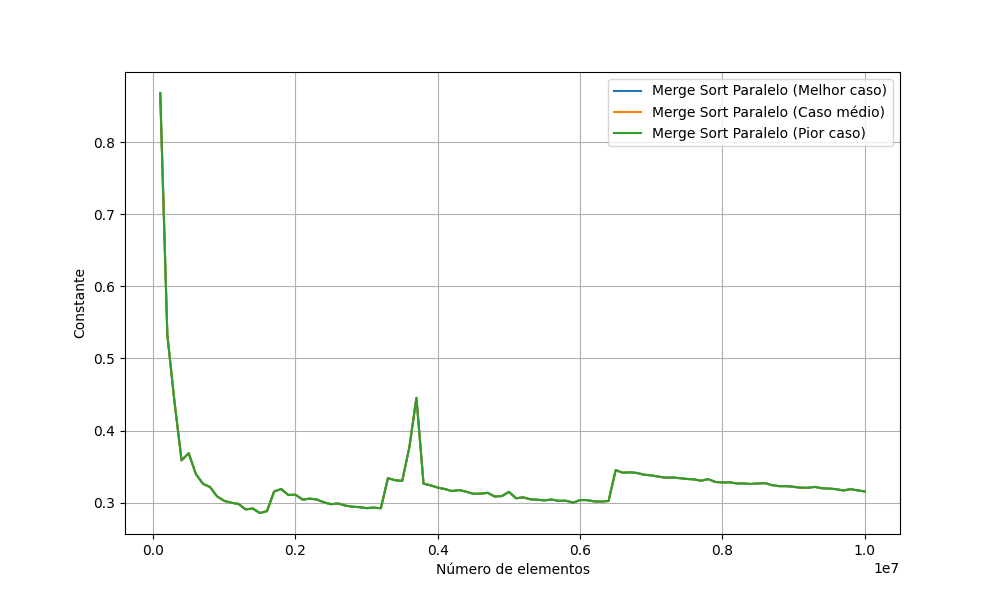
\includegraphics[width=\linewidth]{complexity_descending_parallel_mergesort.png}
        \label{fig:imagem3}
    \end{subfigure}
    \label{fig:desc_c}
\end{figure}

\begin{figure}[H]
    \caption{Constante do Merge Sort com dados aleatórios}
    \centering
    \begin{subfigure}{0.49\textwidth}
        \centering
        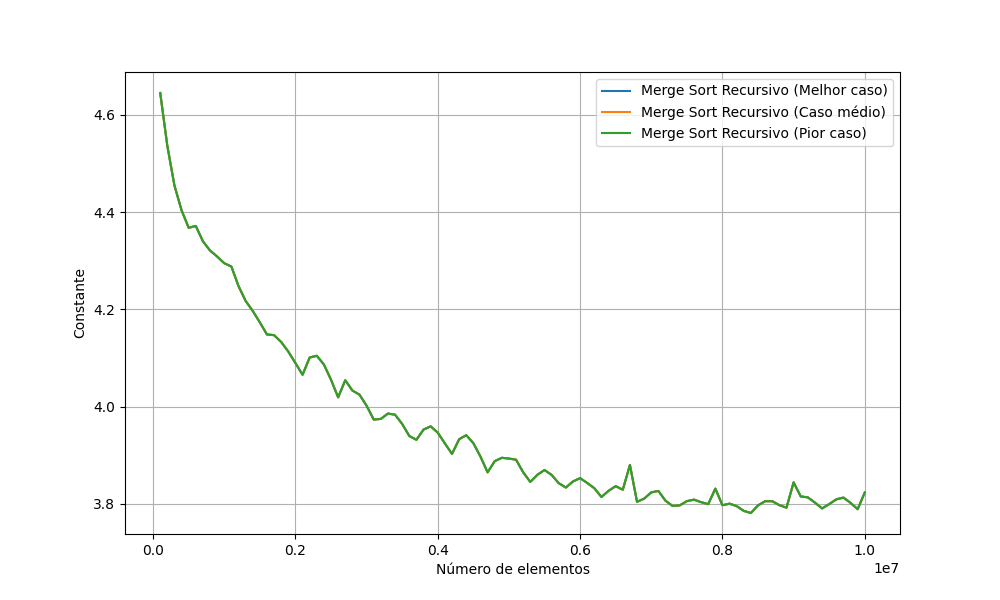
\includegraphics[width=\linewidth]{complexity_random_recursive_mergesort.png}
        \label{fig:imagem1}
    \end{subfigure}
    \hfill
    \begin{subfigure}{0.49\textwidth}
        \centering
        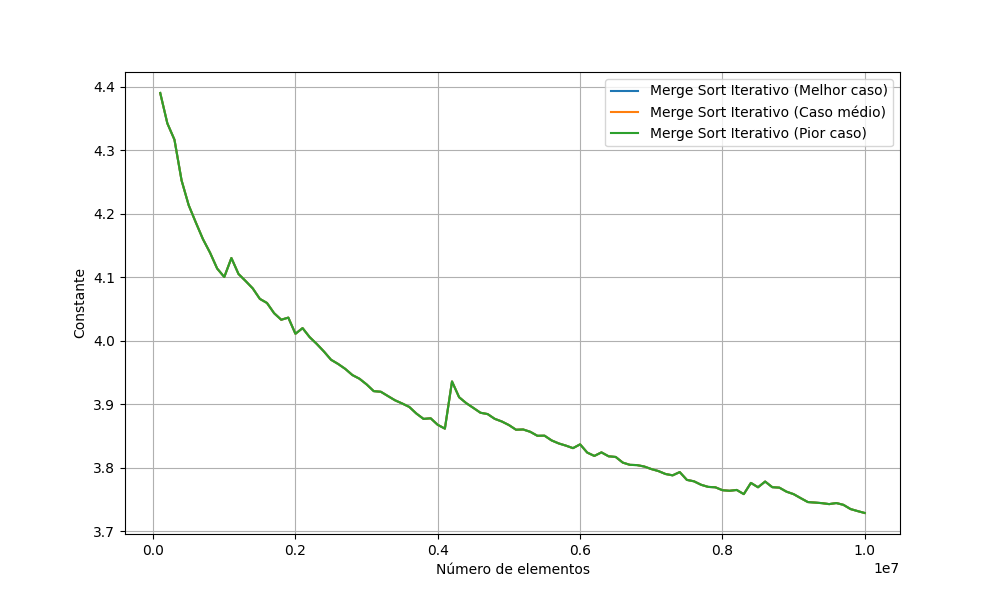
\includegraphics[width=\linewidth]{complexity_random_iterative_mergesort.png}
        \label{fig:imagem2}
    \end{subfigure}
    \begin{subfigure}{0.49\textwidth}
        \centering
        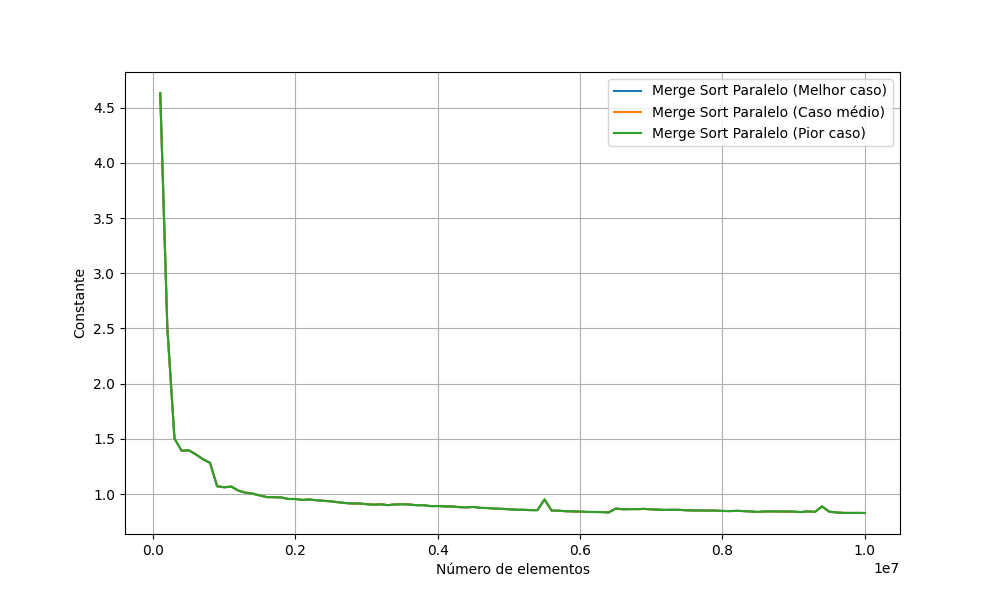
\includegraphics[width=\linewidth]{complexity_random_parallel_mergesort.png}
        \label{fig:imagem3}
    \end{subfigure}
    \label{fig:random_c}
\end{figure}

\section{Conclusão}

Nesse trabalho, analisamos o algoritmo Merge Sort em suas diferentes implementações — recursiva, iterativa e paralelizada — e discorremos sobre como cada uma delas apresenta características específicas que as tornam adequadas para contextos variados. Ademais, ao compararmos o Merge Sort com outros algoritmos de ordenação, como Insertion Sort, Quicksort e o híbrido Quicksert, percebeu-se que cada algoritmo possui suas vantagens e suas desvantagens em diferentes cenários, destacando a importância de considerar as características dos dados e o contexto de aplicação ao selecionar um algoritmo de ordenação.

\section{Referências}
\renewcommand{\baselinestretch}{1.5}

\setlength{\parindent}{0pt}

\hangindent=0.5cm
A New Optimized Version of Merge Sort.  (2023). doi: 10.1109/icetet-sip58143.2023.10151579

\hangindent=0.5cm
BENTLEY, Jon Louis. Programming Pearls, (1989).
 
\hangindent=0.5cm
CORMEN, Thomas H. et al. Introduction to algorithms. MIT press, 2022.

\hangindent=0.5cm
Mutaz, Rasmi, Abu, Sara., Mohammad, F., J., Klaib., Masud, Hasan. Ems: an enhanced merge sort algorithm by early checking of already sorted parts.  (2019).;5(2):15-25. doi: 10.15282/IJSECS.5.2.2019.2.0058

\hangindent=0.5cm
Singh, Jaiveer., Singh, Raju. Merge Sort Algorithm. International Journal of Research, (2014).;1(10):1203-1207.
 
 
\end{document}
